\begin{figure}[h]
	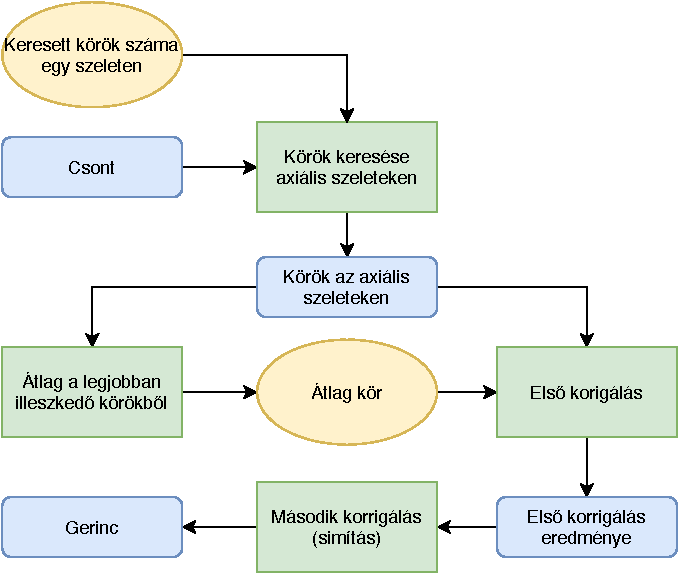
\includegraphics{gerinc_kinyeres.pdf}
	\centering
	\caption{Gerinckijelölés lépései} \label{fig:gerinc_ki}
\end{figure}

\begin{figure}[!tbp]
	\centering
	\begin{minipage}[b]{0.3\textwidth}
		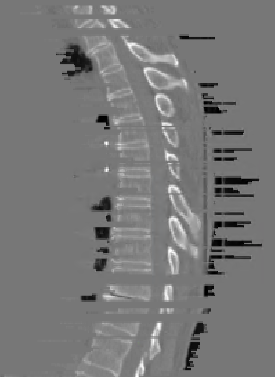
\includegraphics[width=\textwidth]{korrig_0_60}
		\caption{Korrigálatlan}
	\end{minipage}
	\hfill
	\begin{minipage}[b]{0.3\textwidth}
		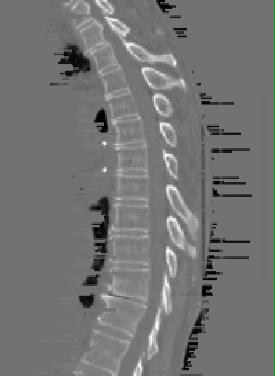
\includegraphics[width=\textwidth]{korrig_1_60}
		\caption{Első korrigálás}
	\end{minipage}
	\hfill
	\begin{minipage}[b]{0.3\textwidth}
		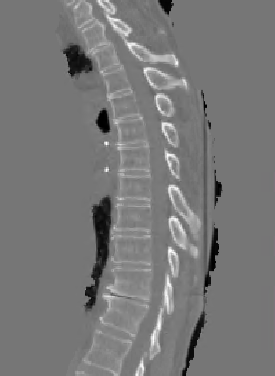
\includegraphics[width=\textwidth]{korrig_2_60}
		\caption{Második korrig}
	\end{minipage}
\end{figure}

%------------------------------------------------------------